\documentclass[11pt,letterpaper]{article}

\usepackage{fancyhdr}
\usepackage[hmargin=2cm,vmargin=2.5cm]{geometry}
\usepackage{graphicx}
\usepackage{amsmath}
\usepackage{amsfonts}
\usepackage{amssymb}
\usepackage{hyperref}
\usepackage{braket}
\usepackage{float}
\usepackage{longtable}
\usepackage{listings}

\pagestyle{fancy}
\setlength\parindent{0in}
\setlength\parskip{0.1in}
\setlength\headheight{15pt}

\lhead{\textsc{John Golden}}
\rhead{\textsc{A Research Note}}
\rfoot{\textsc{\thepage}}
\cfoot{}
\lfoot{\textit{Updated: \today}}

\setcounter{secnumdepth}{0}

\begin{document}

In this note we have some simple Markdown examples and show their conversion to PDF via LaTeX.

\subsection{Handling sections}
Use H1 (\#) for the title, and then H2 (\#\#) for sections.
H2 headers start at the \texttt{subsection} level, and are not numbered.
H3 headers (\#\#\#) and lower just get turned into \texttt{paragraph}s.

\subsubsection{A subsection}
Here's a subsection.

\paragraph{A subsubsection}
... is now a \texttt{paragraph} environment.

\subsection{Equations}
Here's an inline equation: \(E = mc^2\).

Here's a regular equation:
\begin{equation}
    -\frac{\hbar^2}{2m}\nabla^2\psi(r,t) + V(r)\psi(r,t) = i\hbar \frac{\partial}{\partial t}\psi(r,t)
\end{equation}
For multi-line equations, you can use the \texttt{align} environment (or \texttt{gather}, or \texttt{eqnarray}, etc...) like this:
\begin{align}
    a & = b + c \\
    x & = y - z
\end{align}
Unfortunately the raw LaTeX doesn't render in most Markdown previewers, e.g. VSCode.
However, for reasons that are mysterious to me, the VSCode Markdown previewer does allow for newlines via \texttt{{\textbackslash}{\textbackslash}} in equation mode. So if you want to do multiline like that to start, and then switch to the \texttt{align} environment manually before compiling to LaTeX/pdf, go for it.

Note that you don't need to add a blank line before a full-line equation in the Markdown file, e.g. you can write
\begin{lstlisting}
    some text
    
    $$
    1+1=2
    $$
\end{lstlisting}
instead of
\begin{lstlisting}
    some text
    
    $$
    1+1=2
    $$
\end{lstlisting}
And here's a matrix:
\begin{equation}
    A = 
    \begin{pmatrix}
        2 & -1 &  0 & 0 \\
        -1 &  2 & -1 & 0 \\
        0 & -1 &  2 & -1 \\
        0 &  0 & -1 & 2 \\
    \end{pmatrix},~~~
    b = 
    \begin{pmatrix}
        1 \\ 1 \\ 0 \\ 0
    \end{pmatrix}.
\end{equation}

\subsection{Inline code}
Here's some \texttt{inline code}.

\subsection{Lists}
Here's a simple list:
\begin{itemize}
    \item x
    \item y
    \item z
\end{itemize}
Here's an enumerated list:
\begin{enumerate}
    \item x
    \item y
    \item z
\end{enumerate}
Here's an enumerated list with an equation:
\begin{enumerate}
    \item x
    \item y
    \item an equation:
\end{enumerate}
\begin{equation}
    a+b
\end{equation}
\begin{enumerate}
    \def\labelenumi{\arabic{enumi}.}
    \setcounter{enumi}{3}
    \item z
\end{enumerate}

\subsection{Tables}
Here's a simple table. Something is a little off with the rendering, not sure why...
\begin{longtable}[]{@{}ll@{}}
    \hline
    Syntax & Description\tabularnewline
    \hline
    \endfirsthead
    Header & Title\tabularnewline
    Paragraph & Text\tabularnewline
    \hline
\end{longtable}

\subsection{Figures}
Here's a figure with a caption:
\begin{figure}
    \centering
    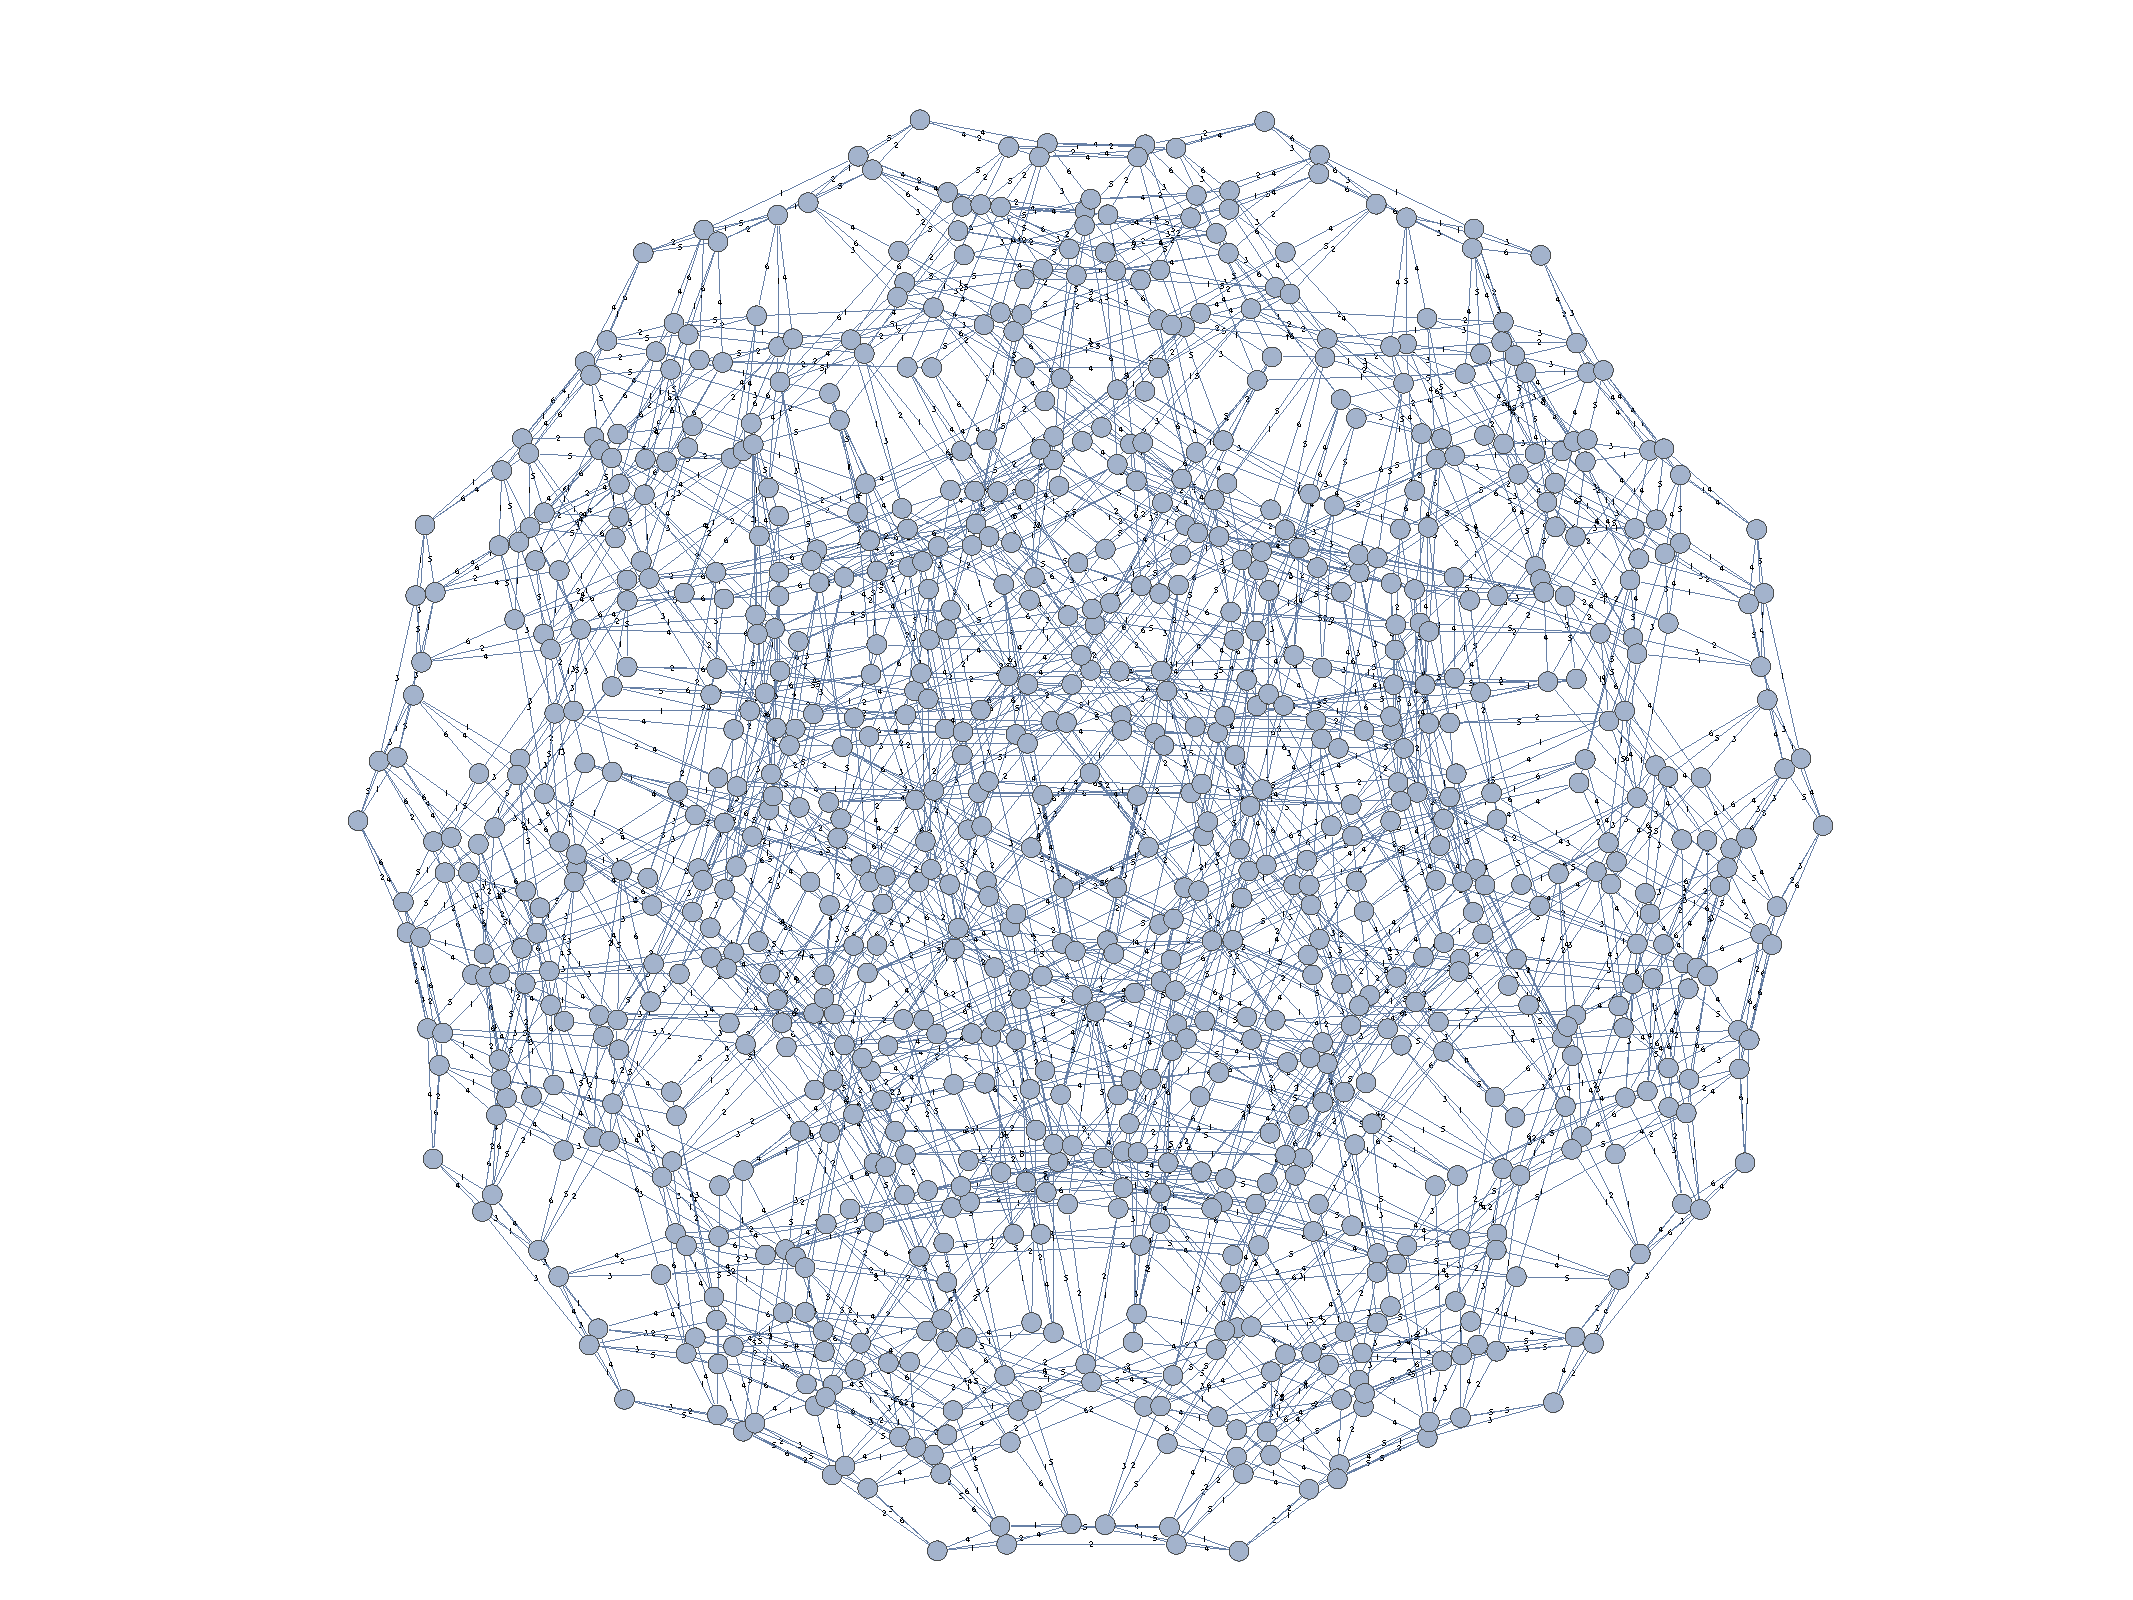
\includegraphics[width=0.8\textwidth]{fig1.pdf}
    \caption{A caption}
\end{figure}



\end{document}